\chapter{Related work} \label{chap3}

\section{Bibliographical research methodology} \label{3biblio_research}

To define the state-of-the-art for ECG classification and Edge Computing. I performed a reduced Systematic Review. The latter is defined as \cite{systematic_review} a 'process of critically evaluating, summarizing, and seeking to reconcile the evidence.' In other words, it is a complete evaluation of literature that differs from a traditional review in that it is undertaken in a methodical (or systematic) manner, following a pre-specified process to avoid bias, with the goal of synthesizing the information gathered. 

Then the first step to perform the systematic review (SR or bibliographical research) was to decide the reference and citation databases to use. In the table \ref{table:dbs_sr} are written the academic search engines used to retrieve the related documents.

\begin{table}[H]
\begin{center}
% \resizebox{\textwidth}{!}{
\begin{tabular}{||p{0.2\linewidth} || p{0.55\linewidth} | p{0.15\linewidth}||}
 \hline
\textbf{Search Engine} & \textbf{Definition} & \textbf{Link} \\ [0.4ex] 
 \hline\hline
Google Scholar & A free web search engine that indexes the full text or metadata of scholarly literature from a variety of publishers and fields. & \href{https://scholar.google.com/}{Link to GS} \\
\hline
PubMed.gov & Contains almost 34 million citations from MEDLINE, life science journals, and online books for biomedical literature. & \href{https://pubmed.ncbi.nlm.nih.gov/}{Link to PM} \\
\hline
IEEEXplore & A research database that allows users to access journal articles, conference proceedings, technical standards, etc. in computer science, electrical engineering, and electronics. & \href{https://ieeexplore.ieee.org/Xplore/home.jsp}{Link to IE} \\
\hline
Scopus & Has a huge collection of Physical Sciences and Engineering papers, from foundational science to novel and unique research, and spanning many disciplines both theoretical and applied. & \href{https://www.sciencedirect.com/}{Link to SCs} \\
\hline
Web Of Science & It is the most reliable publisher-independent worldwide citation database in the world. & \href{https://clarivate.com/webofsciencegroup/solutions/web-of-science/}{Link to WoS} \\
\hline
Papers with code & Their goal is to provide a free and open library that includes Machine Learning articles, code, datasets, methodologies, and evaluation tables. & \href{https://paperswithcode.com/}{Link to PwC} \\
\hline\hline
\end{tabular}
% }
\end{center}
\caption{Databases (search engines) used to find documents}
\label{table:dbs_sr}
\end{table}

Each one of the search engines showed in the previous table work based on a "query" which will contain the information of the topic desired. Besides, to get better results, it is recommended to use multiple queries that may enrich the matter in research. Those queries are listed below, grouped by the specific topic to be found about:

\begin{enumerate}
    \item \textbf{Edge Computing Generalities}: To retrieve the conceptual definition and approximations of Edge Computing I used the following queries:
    \begin{itemize}
        \item Edge Computing arrhythmia
        \item Edge Computing ECG
        \item Edge Computing healthcare arrhythmia
        \item Edge Computing healthcare iot
        \item Edge Computing IoT ecg
        \item Edge Computing healthcare low power mobile
        \item Edge Computing PhysioNet
        \item Edge Computing TensorFlow Lite
    \end{itemize}
    \item \textbf{Options for ECG classification}: To get the different methods used along the history in the ECG classification theme I employed the next queries:
    \begin{itemize}
        \item Machine Learning ECG arrhythmia
        \item Deep Learning ECG arrhythmia
        \item Machine Learning IoT ECG arrhythmia
        \item Deep Learning IoT ECG arrhythmia
    \end{itemize}
    
    As I am going to use Federated Learning technique for edge computing, I employed these techniques. 
    
    \item \textbf{Non-IID Methods}: To evaluate the different methods to deal with Non Independent Nor Identical distributed (Non-IID) data, I search over the following queries:
    \begin{itemize}
        \item Federated learning non iid
        \item Federated learning independent identically distributed
    \end{itemize}
    \item \textbf{Imbalanced data}: To check the techniques used by other authors regarding the class (labels, response variable) imbalanced, I used the next queries:
    \begin{itemize}
        \item Imbalanced data ecg
        \item Imbalanced data federated learning
    \end{itemize}
    \item \textbf{Metrics}: To gather the most used metrics in both ECG and Federated Learning ECG classifications I employed the following queries:
    \begin{itemize}
        \item Federated learning metrics
        \item ECG classification metric
    \end{itemize}
    \item \textbf{Federated learning types}: To understand the possible architectures of Federated Learning I was based on the next queries:
    \begin{itemize}
        \item Federated learning architecture
        \item Types federated learning
    \end{itemize}
    \item \textbf{Arrhythmia types}: To know the different arrhythmia classifications, I employed the following query:
    \begin{itemize}
        \item Cardiac Arrhythmia types
    \end{itemize}
\end{enumerate}


2480 articles were found using the queries mentioned previously. It is important to mention that for each one of those queries, I downloaded the results retrieved in BibTex and CSV formats, depending on the search engine used. With the files saved it was possible to retrieve some generalities from the documents. As an example, in figure \ref{fig:timeline_papers} it is depicted the number of papers found in each search database divided by publication year.

 \begin{figure}[H]
\centering
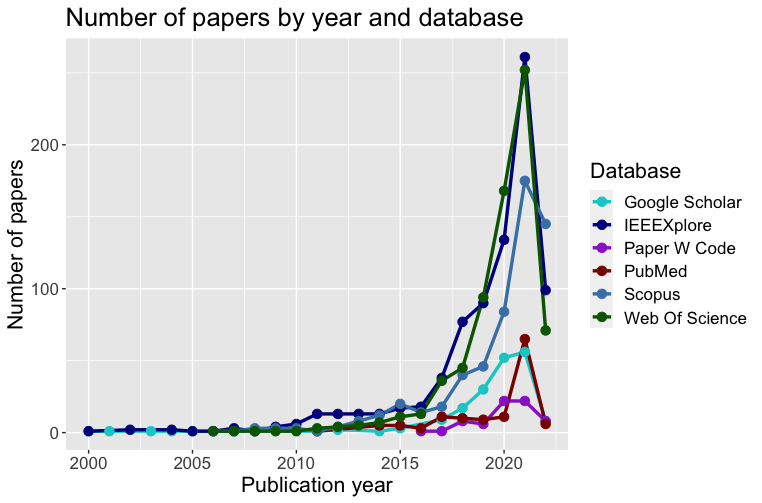
\includegraphics[scale=0.54]{img/timeline_papers.png}
\caption{PRISMA flow for gathering documents}
\label{fig:timeline_papers}
\end{figure}


From the previous graph we can see that most of the papers were published after 2017-2018. At the same time we can see that most of them got published in peak on 2021. ECG classification is a topics that has been worked back in the 2000s. Moreover, the search engine that produced the highest number of resources was IEEEXPlore. 


\section{ECG classification} \label{3state_art_ECG}

After reading the aforementioned documents which was already screened, I gather some relevant highlights regarding the classification of ECG signals. Along the following paragraphs I summarize the most important findings at each topic.

\subsection{Techniques to handle imbalanced data}

In general, imbalanced data describes datasets in which the target class has an unequal distribution of observations. For example, when one class label has a large number of observations while the other has a small number.The authors who have dealt with this topic followed different paths to tackle this issue. Authors from \cite{imbalance_data1} introduced a \textit{Balanced Accuracy (BACC)} and the \textit{Matthew’s Correlation Coefficient (MCC)} to correct the fact that the classes don't share a similar distribution. In the article \cite{imbalance_data2} it was introduced the \textit{Generative Adversarial Network (GAN)} which deals with imbalanced data by generating and using additional fake data for detection purpose. In addition, \cite{imbalance_data3} used the \textit{Synthetic Minority Oversampling Technique (SMOTE)}, which is an oversampling technique. 

Other approaches also include the so-called \textit{Ratio Loss} (\cite{imbalance_data4}) where the global node estimates the composition data each round. When detecting an imbalanced composition continuously, the system acknowledges the class imbalance and load the Ratio Loss. One final possibility is the \textit{Recall of data} in which one randomly augment the lower class and in each training epoch change the selected individuals. Then, there are enough possibilities tried in the literature, each of of them with their pros and cons that can be verified further.


\subsection{Methods for ECG classification} \label{methods_ECG_class}

Along the literature I could find that a huge amount of diverse techniques have been applied when classifying ECG' arrhythmias. As an example \cite{ecg_methods1}, \cite{ecg_methods2}, and \cite{ecg_methods3} focused their efforts on Using Deep Neural Networks (Artificial Neural Networks and Multi-layer Perceptron) to get a model that predicts the abnormality given the ECG signal. In comparison, the author of \cite{ecg_methods4} combined in his paper the use of Naïve Bayes, Adaboost, Random Forest and Support Vector Machines to get the best classifier for his paper. Finally, \cite{ecg_methods5}, \cite{ecg_methods6} and \cite{ecg_methods7} employed in their research some Convolutional Neural Network approaches. Among them the highlighted Squeezenet, Attention mechanism and Resnet as the champion methods to deal with the ECG detection.

 \begin{figure}[H]
\centering
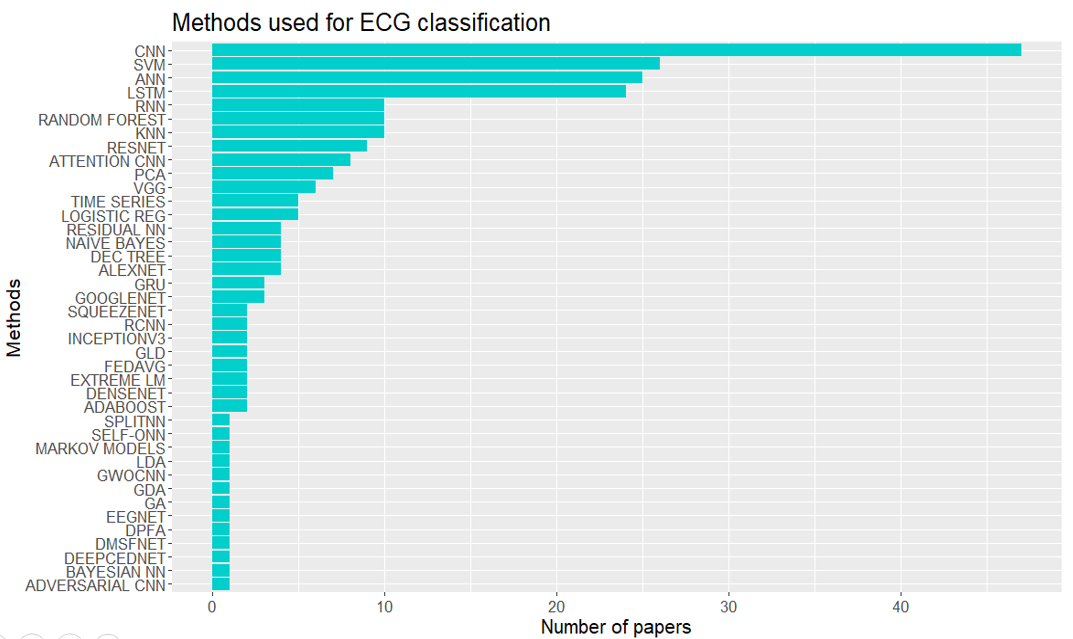
\includegraphics[scale=0.48]{img/classif_methods.PNG}
\caption{Most used classification methods for ECG}
\label{fig:classif_methods}
\end{figure}

As depicted in figure \ref{fig:classif_methods}, the most used technique is the Convolutional Neural Network (CNN). That one includes also some self-made Deep Neural Networks (DNN). On the second place we find Support Vector Machines (SVM) and Artificial Neural Networks (ANN). An very close to them most of the author also used Long-Short Term Memory (LSTM) algorithms. On the opposite, a few papers contributed with techniques like GWOCNN, DFPA, DEEPCETNET, etc, which are also CNN but that have specific alterations adapted to by the papers' authors.

\subsection{Metrics for ECG classification}\label{chap3metrics}

With respect to ECG arrhythmia classification, there are plenty of measurements employed in the literature. In figure \ref{fig:metrics_ECG} I show the most relevant metrics used in this aim, gathered from the available articles and papers shown in chapter \ref{3biblio_research}. 

 \begin{figure}[H]
\centering
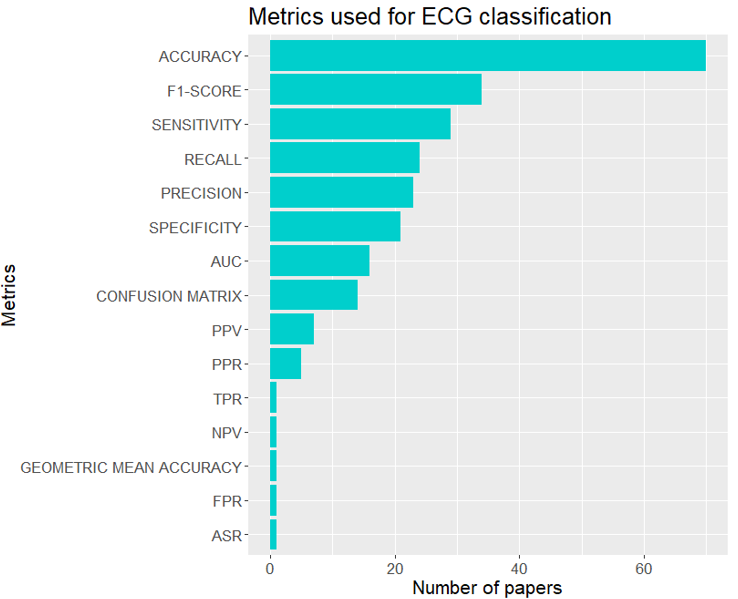
\includegraphics[scale=0.48]{img/metrics_ECG.PNG}
\caption{Most used metrics for ECG}
\label{fig:metrics_ECG}
\end{figure}

From the previous chart it is evident that the most used measure is the \textbf{Accuracy}. In the second place, the \textit{F1-Score} is often used. It is important to clarify that the latter is preferred when dealing with unbalanced data, since it take into account both \textit{Recall} and \textit{Precision} for its calculation. Some papers that consider the 4 mentioned measures at the same time can be found in \cite{metrics_ecg1}, 
\cite{metrics_ecg2} and \cite{metrics_ecg3}.


\subsection{Edge computing using Federated Learning} \label{fedrated_learning_as_edge computing}

To understand how we can we use Fedrated learning as Edge computing. This paper \cite{fedrated_learning_as_edge_computing} is published on 2021 which states that Federated Learning is a machine learning scheme in which a shared prediction model can be collaboratively learned by a number of distributed nodes using their locally stored data. It can provide better data privacy because training data are not transmitted to a central server. Federated learning is well suited for edge computing applications and can leverage the the computation power of edge servers and the data collected on widely dispersed edge devices.

Edge federated learning solves the data island problem by fully exploring the huge potential of the data on terminal devices like mobiles or small iot devices without infringing on user’s privacy, and it greatly improves the efficiency of model learning in edge computing systems usually edge server.  Therefore, it can be widely used in many scenarios where privacy protection and resource utilization are critical. It can apply to healthcare system, vehicular network and intelligent recommendation. 


\subsection{Methods to handle NON-IID data} \label{non_iid_handling}

Along the literature, the researches performed have been focused on tackling the Non Independent Nor Identical distributed (Non-IID) problem that make the models in FL under-perform. In the following part I present a summary of the most relevant techniques used to deal with the mentioned issue.

\textbf{Over/under-sampling}: This is one of the most common techniques used to balance the data. It consist of randomly creating (or removing) data to equate distributions. The simplest way to do it is called Random Oversampling (ROS). The latter is the process of randomly picking and replacing instances from the minority class in the training dataset. There are other techniques like SMOTE \cite{metrics_ecg1}. SMOTE is a data augmentation algorithm that creates synthetic data points depending on the original data points. The technique can be thought of as a more advanced variant of oversampling or as a specific data augmentation process. SMOTE has the advantage of not creating duplicate data points, but rather synthetic data points that are somewhat different from the original data points \cite{imbalance_data3}.

\begin{figure}[H]
\centering
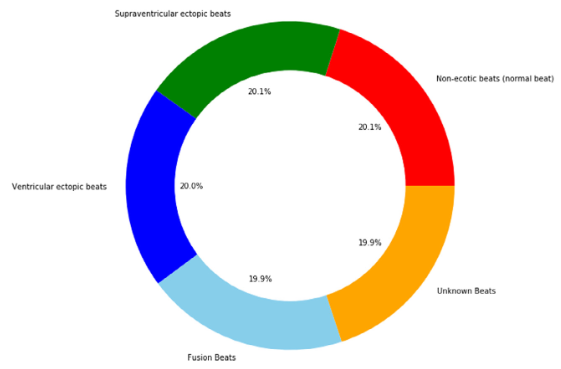
\includegraphics[scale=0.6]{img/metrics_ecg1_ROS.PNG}
\caption{The distribution of the up-sampled (re-balanced) dataset. \cite{metrics_ecg1}}
\label{fig:metrics_ecg1_ROS}
\end{figure}



\textbf{Data sharing strategy}: In the paper \cite{fl18} they showed that for neural networks trained with highly skewed non-IID data, where each client device trains just on a single class of data, the accuracy of federated learning drops by up to 55\%. They also showed that the weight divergence, which can be measured by the Earth mover's distance (EMD) between the distribution over classes on each device and the population distribution, can explain the loss in accuracy. As a solution, the proposal was to establish a limited sample of data that is globally shared across all edge devices to improve training on non-IID data. Their proposed data sharing is exposed in the following image:

\begin{figure}[H]
\centering
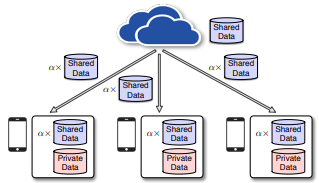
\includegraphics[scale=0.9]{img/fl18_datasharing.PNG}
\caption{ Illustration of the data-sharing strategy. \cite{fl18}}
\label{fig:fl18_datasharing}
\end{figure}





\textbf{Fedprox}: FedProx uses Federated Average Aggregation (FedAvg) to improve the local aim. It restricts the size of local updates directly. To limit the distance between the local model and the global model, it adds an additional L2 regularization term to the local objective function. This is a simple approach to keep the local updates under control so that the averaged model stays close to the global optima. To regulate the weight of the L2 regularization, a hyper-parameter is introduced \cite{fl19}.

\subsection{Metrics for Federated Learning}

Inside the FL framework the same metrics showed in \ref{chap3metrics} are often used. In the ECG case, metrics like Accuracy, F1-Score, Recall and Precision are usually employed to measure the overall capacity of the model to detect the diagnoses. I will be usually using the same metrics to evaluate the performance of the each node which can be acting as edge server(global node) or edge node(local node). 


\subsection{PhysioNet/Computing in Cardiology Challenge 2020}

\subsubsection{Introudction and Keypoints}

As I am going to use \cite{physionet_challenge_2020} PhysioNet/Computing in Cardiology Challenge 2020 dataset. It is often good to consider and finding out what papers has been published and what kind of architecture they were following. 

\cite{main_arythmia_detection}To encourage more multidisciplinary researches, PhysioNet in Cardiology Challenge 2020 (Challenge 2020) \cite{physionet_challenge_2020} provided high-quality 12-lead ECG data obtained from multiple centers with a large set of cardiac abnormalities. The aim of Challenge 2020 was to identify clinical diagnoses from 12-lead ECG recordings, providing an opportunity to employ various advanced methods to address clinically important questions that are either unsolved or not well-solved \cite{arythmia_detection_9}.

Later I did the specific analysis specifically considering the papers published during conference. 41 teams got selected during this challenge and others are simply discarded because the method did not work on the hidden set, the team failed to submit a preprint or a final article on time, or the team was absent during CinC conference. Looking at the 41 teams papers published in PhysioNet \cite{physionet_challenge_2020}. One can observe that some techniques are used by the majority of the teams. The results indicate that ECG classification is a complex process that includes multiple techniques. Among these techniques, signal processing, DNNs, convolutional neural networks (CNNs), end-to-end and multi-binary classifications are used by all of the top 10 teams. In addition, there are several important points 1) deep-learning methods were more popular than traditional methods in Challenge 2020; 2) all the teams that employed deep-learning methods used CNNs; and 3) none of the top-10 teams used hand-labeled features (except demographic features); they all adopted end-to-end models instead. 

To investigate the techniques applied by each team, I considered five aspects of the methods that formed a solution pipeline (see \ref{fig:meta_analysis_2020_teams}): data preprocessing, feature engineering, machine-learning models, training strategy, and applications to the real world. Table 2 presents these five aspects.


\begin{figure}[H]
\centering
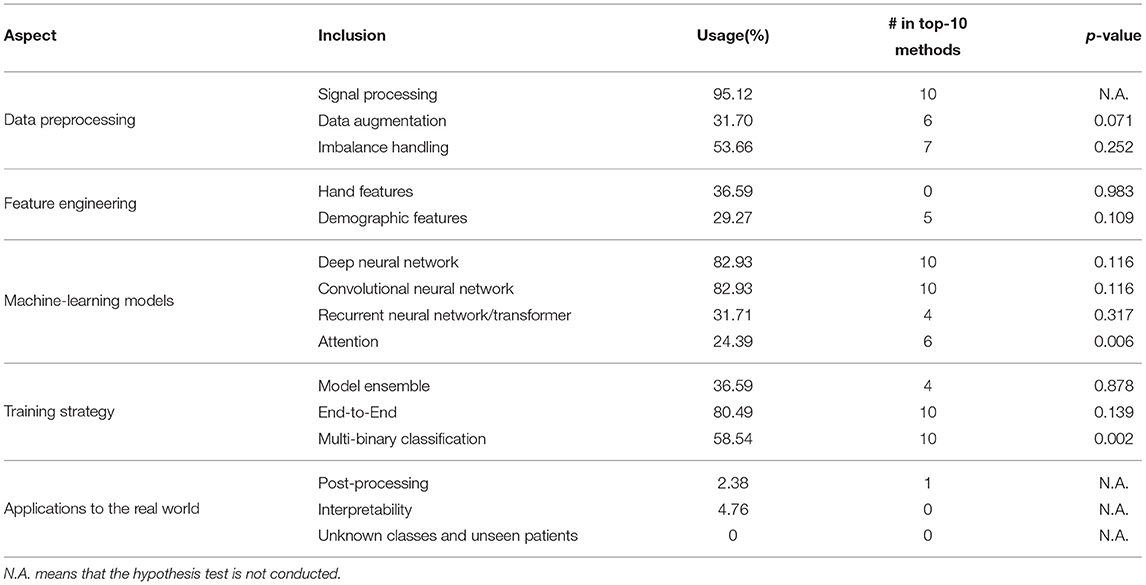
\includegraphics[scale=0.32]{img/meta_analysis_2020_teams.jpeg}
\caption{Details of employed techniques.}
\label{fig:meta_analysis_2020_teams}
\end{figure}


\cite{main_arythmia_detection} One can also notice that the three highest-ranking teams used the model ensemble \cite{first_team, second_team, third_team}, but only 14 out of 41 teams employed this strategy. It is also important to note that model ensemble only helps if used for single model rather than models that are structurally different. Most of team also used only age and sex as features rather other using demographic features or 12-lead ECG based features. The training data in Challenge 2020 suffer from heavy class imbalance (as shown in \ref{fig:label_ditro_alldata}) so most teams used  threshold optimization \cite{eighth_team, second_team, ninth_team} and weighted loss \cite{sixth_team, seventh_team} to handle imbalance class issue. In addition, over-sampling \cite{thirteen_team}, down-sampling \cite{sixteen_team}, and other methods have been employed in Challenge 2020.

\subsubsection{Practical Lessons:}

\begin{enumerate}
  \item Data augmentation should be employed and adapted to specific scenarios.
  \item Combining different features can improve performance.
  \item A hybrid design of different types of deep neural networks (DNNs) is better than using a single type.
   \item The use of end-to-end architectures should depend on the task being solved.
   \item Multiple models are better than one.
\end{enumerate}

\subsubsection{Finding open source algorithms from Published Papers}

To find open source code of the papers I have search them in Google and Github, I was able to find the source code of 9 papers that was accepted during the challenge including team 2, team 6 and team 20. I will be later using these source code for analysis try to incorporate some additional features that i have identified during centralized learning approach of Fedarated learning. 

It is important to note that \textbf{Pytorch} is most widely used framework by participants implementation of the Physionet Challenge 2020. [\ref{fig:framework_used_by_2020_teams}]. 'Not Mentioned' either represents that they didn't wrote in their paper what kind of implementation they are following or I am not able to find out their implementation of the paper on the internet. 

\begin{figure}[H]
\centering
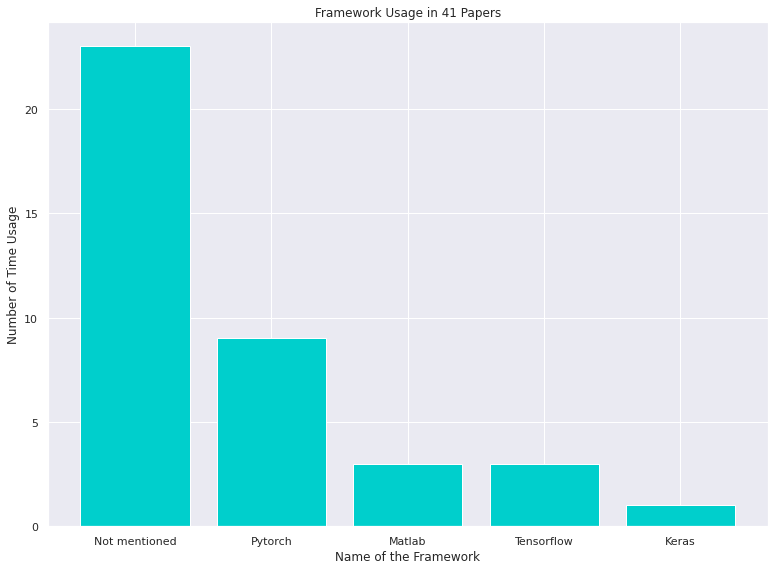
\includegraphics[scale=0.5]{img/framework_usage_in_papers.png}
\caption{Most used framework during Physionet Challenge 2020}
\label{fig:framework_used_by_2020_teams}
\end{figure}

I have also created an excel sheet which has combination of the meta analysis of 2020 challenge \cite{main_arythmia_detection} and all the open source code related to each team participated in the challenge. Which can be found here: https://bit.ly/3bgFtWs 

